\documentclass[12pt]{article}
\usepackage{enumitem}
\usepackage{setspace}
\usepackage{graphicx}
\usepackage{subcaption}
\usepackage{amsmath, amsthm}
\usepackage{float}
\usepackage{booktabs}
\RequirePackage[colorlinks]{hyperref}
\usepackage[lined,boxed,linesnumbered,commentsnumbered]{algorithm2e}
\usepackage{xcolor}
\usepackage{listings}
\lstset{basicstyle=\ttfamily,
  showstringspaces=false,
  commentstyle=\color{red},
  keywordstyle=\color{blue}
}
\graphicspath{ {../plots} }


% Margins
\topmargin=-0.45in
\evensidemargin=0in
\oddsidemargin=0in
\textwidth=6.5in
\textheight=9.0in
\headsep=0.25in

\linespread{1.1}

% Commands
\newenvironment{solution}
  {\begin{proof}[Solution]}
  {\end{proof}}

\title{NFL 3rd Down Conversion and Income Prediction }
\author{Daniel Lin}

\begin{document}

\maketitle

\section{Introduction}

The purpose of this report is to evaluate how machine learning algorithms and techniques can influence model performance. The five machine learning algorithms we analyze are: Decision Trees, K Nearest Neighbors, Support Vector Machines, Boosting, and Neural Networks.  The classification problems are stated in the section below.

\subsection*{NFL Third Down Conversion}

In American football, there are four downs to convert 10 yards. Given that fourth downs will commonly result in a field goal or punt, third down conversions are extremely vital.  There are a multitude of factors that can influence the probability of conversion e.g. yards to go, pass play, rush play, weather, or simply having an all-star QB. Given the recent shift towards analytics in the field, this seems to be an interesting classification problem. In game, announcers will commonly say "The analytics say: X\% conversion rate for this team." I think we can do better than a univariate summary statistics. Even given near perfect scenarios, there is always something that can go wrong.

The features used for this dataset are:  yards to-go, formation, play type (rush, pass, pass type, rush direction), yard line, quarter, time left in quarter, offense team, and defensive team.

\subsection*{US Income}
The other classification problem utilizes data from US Census Bureau in 1994 in order to predict if an individual made more than \$50,000 (roughly \$100,000 in 2023). I thought this would be an interesting dataset to understand the dynamic of 
income inequality. Given the complexity of income, this would also be helpful to analyze overfitting and the non-linear relationships between features and the output. 

The features used for this dataset are: age, working class, education, marital status, occupation, relationship, race, gender, capital gain, capital loss, work hours per week, and native country.

\section{Methodology}
\subsection*{Modeling}
The primary machine learning library in this report is Sci-kit learn in Python. Since the focus was analysis, this was a great library to iterate on many models and metrics, sacrificing some model scalability for ease of implementation. PyTorch was also considered for the Neural Network portion as it has many performance benefits for Deep Learning.

For categorical variables, I transposed the variables to columns and gave them binary indicators. For continuous variables, I used Standard Scaler which subtracts the mean and divides by the standard deviation. This is impactful for many of the algorithms. For K-Nearest Neighbor, scaling helps so that features on a smaller range do not outweigh large numbers.  For SVM, this is necessary for optimization as the algorithm to find the separating hyperplane takes the dot product between the input values and weights which can cause the distances to become extremely large. Neural networks also benefit in both a training and classification performance standpoint.

\subsection*{Analysis}
For each model, I first tuned the hyperparameters of the underlying model.  Given the binary classification problems, I chose AUC (Area Under the Curve) as the main metric to optimize for when tuning the hyperparameters.  AUC is calculated by utilizing the receiver operating characteristic curve. This method plots the False Positive Rate against the True Positive Rate. An AUC of 0.5 can be thought of as good as flipping a coin. The larger the area under the curve, the better the classifier.

For the learning curves, I used Accuracy, which describes how well a classifier performs across the classes. Accuracy can be misleading when datasets are very imbalanced because the majority class may dominate. However, I chose this metric because I wanted to utilize a different metric to learn how imbalance may affect the analysis. The imbalance in the NFL dataset was 39\% and 24\% in the Income dataset.

Other metrics I looked at were: RMSE, Loss, Precision, Recall and F1 Score.  RMSE is commonly used for simple linear regression problems, however, for binary classification, it is not as useful given the continuous and non-directional nature of the metric.

For each analysis, I split the dataset 70/30 for training and validation. I would utilize this split to find the "best model" by iterating a tuning parameter across a range of values, then maximizing the parameter on the validation set. The code iterates through the specified hyperparameters sequentially to optimize for the validation set. After I find the best model, I plot the Learning Curves by using a 5-fold CV method. By increasing the training size, I can evaluate the performance on the validation set. Since the MLP algorithm runs iteratively, instead of analyzing on an increase in training size using 5-fold, I measure the validation error directly on the epochs.

\section{Decision Tree}
For the Decision Tree, we create the decision nodes by using the Gini impurity.  The Gini impurity index is 0 when all inputs are in the same class and 1 when it is evenly split.  The goal is to split on the highest impurities (or lowest index), which improves the model performance and optimization.

For this algorithm, I used a pre-pruning method to minimize overfitting.  I chose this method because I wanted to understand how altering the complexity of the tree would impact overfitting. An alternative would be to use a post-pruning technique such as cost-complexity pruning, however, I thought it would be simpler to visualize limiting the depth over increasing regularization.

\begin{figure}[H]
\begin{subfigure}{0.5\textwidth}
\centering
\includegraphics[width=\linewidth]{/nfl/decision_tree_Depth_AUC.png}
\end{subfigure}%
\begin{subfigure}{0.5\textwidth}
\centering
\includegraphics[width=\linewidth]{/income/decision_tree_Depth_AUC.png}
\end{subfigure}
\end{figure}

In both cases, we can see a sign of overfitting as the depth increases to higher levels. This is shown when as the Training and Validation lines start to diverge. Without the validation curves, it would seem that we should maximize the depth for the best performance, however, this leads to overfitting. I chose the optimal depth as the maximum AUC in the validation set. In the NFL dataset, it overfits sooner at a maximum depth of 6 whereas the Income dataset overfits at 8. 

Other tuning hyperparameters are the minimum number of samples required to split and minimum samples in a leaf node. The more granular a Decision Tree becomes the more likely it results in overfitting. For this analysis, I did not alter these parameters since the Max Depth took those into account indirectly. 

\begin{figure}[H]
\begin{subfigure}{0.5\textwidth}
\centering
\includegraphics[width=\linewidth]{/nfl/decision_tree_accuracy_learning_curve.png}
\end{subfigure}%
\begin{subfigure}{0.5\textwidth}
\centering
\includegraphics[width=\linewidth]{/income/decision_tree_accuracy_learning_curve.png}
\end{subfigure}
\end{figure}

After optimizing for the tree depth, I use 5-fold cross validation to plot model performance (Accuracy) against the training size. Interestingly, we see the accuracy seem to converge in both cases. This may be an indicator that the model does generalize well.  Predicting income seems to have much higher accuracy than predicting a third-down conversion.

\section{K Nearest Neighbor}
For the KNN algorithm, we use uniform weights as we have already scaled our input data. It is intuitive that to some degree, as we increase K, our model becomes more general and that results in less overfitting.

\begin{figure}[h]
\begin{subfigure}{0.5\textwidth}
\centering
\includegraphics[width=\linewidth]{/nfl/knn_n_neighbors_AUC.png}
\end{subfigure}%
\begin{subfigure}{0.5\textwidth}
\centering
\includegraphics[width=\linewidth]{/income/knn_n_neighbors_AUC.png}
\end{subfigure}
\end{figure}

For the NFL Third Down Conversion model, our optimal K is 141. This value of K is extremely large and we can see that the model actually seems to converge much earlier as there is minimal gains pass a certain point. This also hints that  it difficult to classify Third Down conversion with the input data.  For our Income data, our optimal query point is 31, which is more reasonable. Another hyperparameter we alter is the distance metric, which we can choose to be Euclidean or Manhattan distance.  The Euclidean distance may be more sensitive to overfitting since it squares the errors whereas the Manhattan distance looks at the absolute distance. However, when altering these parameters, it made little to no difference and the optimizer chose the Euclidean distance.

\begin{figure}[H]
\begin{subfigure}{0.5\textwidth}
\centering
\includegraphics[width=\linewidth]{/nfl/knn_accuracy_learning_curve.png}
\end{subfigure}%
\begin{subfigure}{0.5\textwidth}
\centering
\includegraphics[width=\linewidth]{/income/knn_accuracy_learning_curve.png}
\end{subfigure}
\end{figure}

In this case, we see that training size has a different impact to the learning curves as with the Decision Tree. In both cases, as our training size increases, both our validation and training accuracy increase. This may be because we get more points that are closer to our query point as the training data increases. We are always limited to K neighbors so as data increases, we may just have closer neighbors overall. 

\section{Support Vector Machine}
The Support Vector Machine looks to find the optimal hyperplane that splits the data. Given this model uses all datapoints to iteratively solve for optimal weights, the increase in training data can hinder model performance, leading to long training times.

For the SVM, our tuning parameter is a regularization constant. Given the tuning parameter, this is a classic example of the variance-bias tradeoff.  A low value of C will result in more penalization for stronger weights, which will decrease variance but increase bias leading to a possibility of underfitting.  With high values of C, we will see less penalization, which will have the inverse effect and a possibility of overfitting. I tested C values of 0.001, 0.01, 0.1, 0.5, and 1.

\begin{figure}[H]
\begin{subfigure}{0.5\textwidth}
\centering
\includegraphics[width=\linewidth]{/nfl/svm_C_AUC.png}
\end{subfigure}%
\begin{subfigure}{0.5\textwidth}
\centering
\includegraphics[width=\linewidth]{/income/svm_C_AUC.png}
\end{subfigure}
\end{figure}

It seems like our model performance flattens out quickly. Another interesting note is that the Validation set actually outperforms the training set in the US income dataset. The NFL dataset had an optimal regularization value of 0.1 whereas the Income dataset was higher at 0.5. This seems to be intuitive as the NFL dataset was more subject to overfitting in some of the other models, like the Decision Tree. This means we would have a more optimal model by utilizing more regularization.

 \begin{figure}[H]
\begin{subfigure}{0.5\textwidth}
\centering
\includegraphics[width=\linewidth]{/nfl/svm_accuracy_learning_curve.png}
\end{subfigure}%
\begin{subfigure}{0.5\textwidth}
\centering
\includegraphics[width=\linewidth]{/income/svm_accuracy_learning_curve.png}
\end{subfigure}
\end{figure}

The accuracy here also seems to converge as we increase our training sample size.

\section{Boosting}
In this section, we utilize the Ada Boosting algorithm, which takes simple decision trees in an ensemble fashion. Boosting is a method that utilizes many weak predictors to create a strong predictor. The reason I chose Ada Boosting over Gradient Boosting is simply because of performance and training time. In my experience, Gradient Boosting can be more rigorous as it requires calculating the gradient at each iteration. For the Ada Boosting algorithm, we alter the number of weak learners to tune our model. 

\begin{figure}[H]
\begin{subfigure}{0.5\textwidth}
\centering
\includegraphics[width=\linewidth]{/nfl/ada_boost_N_estimators_AUC.png}
\end{subfigure}%
\begin{subfigure}{0.5\textwidth}
\centering
\includegraphics[width=\linewidth]{/income/ada_boost_N_estimators_AUC.png}
\end{subfigure}
\end{figure}

For the NFL dataset, the optimal number is 255. For our income dataset, the optimal number is 280.  This means that we used over 250 weak learners to predict an outcome. A decent analogy here would be predicting the outcome of an election of a state.  Let's say we have 250 experts that are good at predicting the outcome on a given slice, let's say age for one, gender for another, and so on. Each expert is good at predicting the outcome for their attribute but not overall. By boosting the predictions of each expert, we can build a comprehensive model. 

 \begin{figure}[H]
\begin{subfigure}{0.5\textwidth}
\centering
\includegraphics[width=\linewidth]{/nfl/ada_boost_accuracy_learning_curve.png}
\end{subfigure}%
\begin{subfigure}{0.5\textwidth}
\centering
\includegraphics[width=\linewidth]{/income/ada_boost_accuracy_learning_curve.png}
\end{subfigure}
\end{figure}

Here, we see the boosting model perform quite well and converge as we increase in training samples.

\section{Neural Network}
For the Neural Networks, I chose a Multilayer Perceptron model as it was the most classical example of a Neural Network. I used the ReLU activation function since it avoids the vanishing gradient problem. I decided to alter the model complexity by specifying more layers in the model to see how it would impact model performance. I iterated on 1 to 4 layers with each layer mapping to 32 to 4 nodes.  

\begin{figure}[H]
\begin{subfigure}{0.5\textwidth}
\centering
\includegraphics[width=\linewidth]{/nfl/mlp_N_hidden_layers_AUC.png}
\end{subfigure}%
\begin{subfigure}{0.5\textwidth}
\centering
\includegraphics[width=\linewidth]{/income/mlp_N_hidden_layers_AUC.png}
\end{subfigure}
\end{figure}

For both datasets, it turns out that the least number of hidden layers had the best performance on the validation set. This is intuitive as increasing model complexity can cause overfitting. 

Another parameter I altered was the Activation function. I tried both ReLU and Sigmoid, in both cases, the ReLU function outperformed the Sigmoid function.

\begin{figure}[H]
\begin{subfigure}{0.5\textwidth}
\centering
\includegraphics[width=\linewidth]{/nfl/mlp_Accuracy_learning_curve.png}
\end{subfigure}%
\begin{subfigure}{0.5\textwidth}
\centering
\includegraphics[width=\linewidth]{/income/mlp_Accuracy_learning_curve.png}
\end{subfigure}
\end{figure}

Since the MLP algorithm runs through the dataset in iterations, we can naturally see how an increase in iterations (epochs) can impact overfitting. In this case, it is interesting to see that the iterations has little to no-affect on the validation set.

\section{Evaluation of Models}
\subsection*{Scalability}
As I stated earlier, the SVM classifier had the most notable performance issues. As you can see below, the training time grows exponentially as the number of training samples increases. In contrast, the Decision Tree classifier tends to 
grow linearly as the number of samples increase.

\begin{figure}[H]
\begin{subfigure}{0.5\textwidth}
\centering
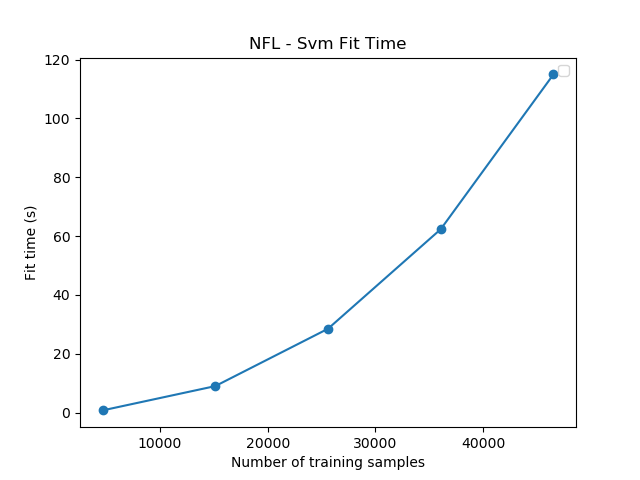
\includegraphics[width=\linewidth]{/income/svm_fit_curve.png}
\end{subfigure}%
\begin{subfigure}{0.5\textwidth}
\centering
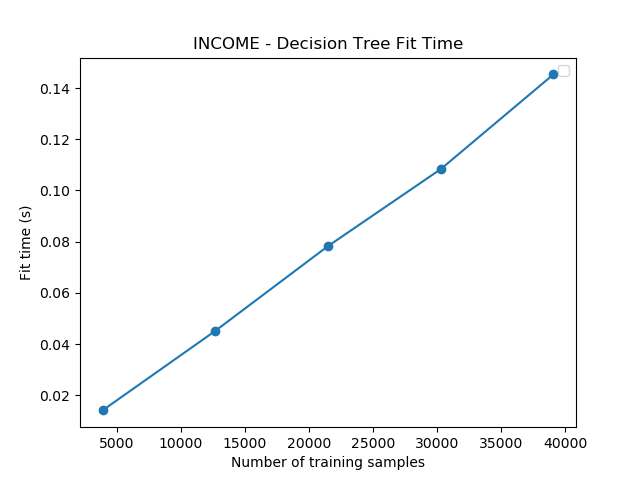
\includegraphics[width=\linewidth]{/income/decision_tree_fit_curve.png}
\end{subfigure}
\end{figure}

The SVM model is very slow given the number of computations it requires to optimize the parameters. When scoring the dataset, the model seemed to grow linearly in the SVM. I chose a simple MLP model, otherwise I think the NN could have also run into some performance issues. 

\begin{figure}[H]
\begin{subfigure}{0.5\textwidth}
\centering
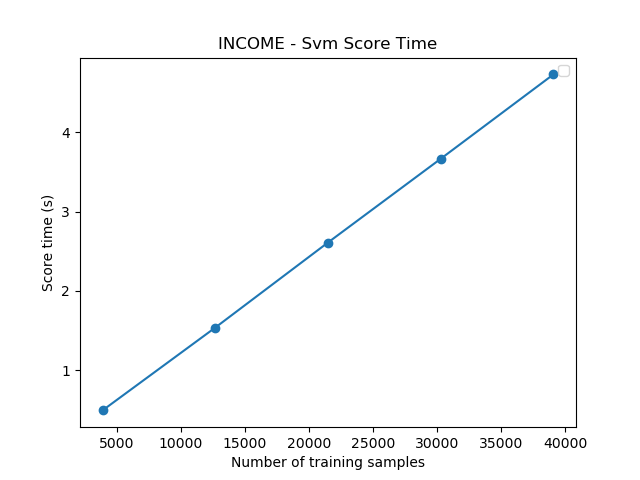
\includegraphics[width=\linewidth]{/income/svm_score_curve.png}
\end{subfigure}%
\begin{subfigure}{0.5\textwidth}
\centering
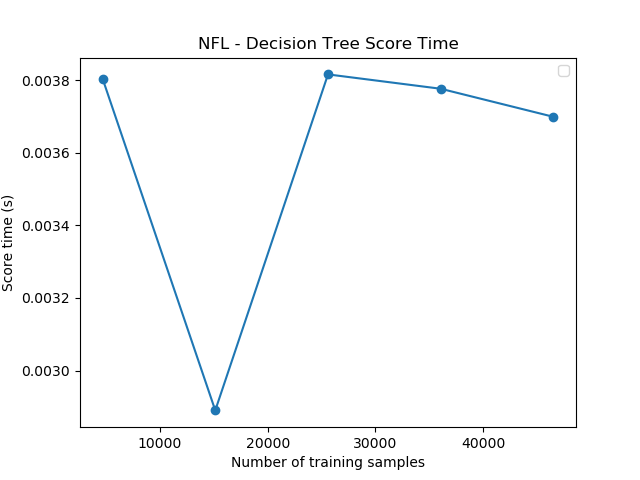
\includegraphics[width=\linewidth]{/income/decision_tree_score_curve.png}
\end{subfigure}
\end{figure}


\subsection*{Classification Performance}

I used four metrics to evaluate the performance.

\begin{itemize}
  \item Precision = $\frac{\text{TP}}{\text{TP} + \text{FP}}$, out of the positive predictions, what percentage are truly positive?
  \item Recall = $\frac{\text{TP}}{\text{TP} + \text{FN}}$, out of the truly positive, what percentage were predicted positive?
  \item F1 Score = Harmonic mean of Precision and Recall, a blended score.
  \item Accuracy = $\frac{\text{Predictive Correctly}}{\text{All Predictions}}$
\end{itemize}

\begin{table}[H]
\caption{NFL Classification Metrics}
\centering
\begin{tabular}{|c|c|c|c|c|}
\hline
\textbf{Algorithm} & \textbf{Precision} & \textbf{Recall} & \textbf{F1-Score} & \textbf{Accuracy} \\ \hline
Decision Tree & 0.574 & 0.525 & 0.549 & 0.668 \\ \hline
KNN & 0.600 & 0.386 & 0.470 & 0.666 \\ \hline
SVM & 0.585 & 0.516 & 0.549 & 0.674 \\ \hline
AdaBoost & 0.597 & 0.479 & 0.532 & 0.676 \\ \hline
MLP & 0.583 & 0.532 & 0.556 & 0.675 \\ \hline
\end{tabular}
\end{table}

Depending on the classification problem, we may want to optimize for Precision vs Recall. For example, when detecting spam, it may be better to focus on precision since we do not want to accidentally send important emails to spam. In contrast, when working on a disease diagnosis, it may be beneficial to optimize for Recall since the consequences are more dire.  In this case, since we are simply interested in classifying if a third down conversion is achieved, we will put our focus on F1-Score and Accuracy. In this dataset, the MLP model seems to have the best all around performance. KNN had the strongest precision but at the sacrifice of recall. This can be intuitive since it may be more "picky" on classification meaning that it doesn't predict as many positives but when it does, it is more sure of it. The boosting algorithm had the highest accuracy but we see that Recall is the second lowest out of the models. This may be due to imbalance in the dataset and the boosting model is good at picking up when a team achieves a first down simply due to some dominating factor, perhaps yards-to-go being one of them. It would be interesting to look at a Partial Dependency plot of this feature to see the marginal contribution to the overall prediction.


\begin{table}[H]
\caption{Income Classification Metrics}
\centering
\begin{tabular}{|c|c|c|c|c|}
\hline
\textbf{Algorithm} & \textbf{Precision} & \textbf{Recall} & \textbf{F1-Score} & \textbf{Accuracy} \\ \hline
Decision Tree & 0.748 & 0.611 & 0.611 & 0.861 \\ \hline
KNN & 0.720 & 0.620 & 0.620 & 0.855 \\ \hline
SVM & 0.740 & 0.601 & 0.601 & 0.858 \\ \hline
AdaBoost & 0.777 & 0.656 & 0.656 & 0.876 \\ \hline
MLP & 0.755 & 0.608 & 0.608 & 0.862 \\ \hline
\end{tabular}
\end{table}

In our Income prediction dataset, our algorithms were much stronger. We see high performance of greater than 0.8 accuracy across all models. The best model in this case is more obvious, in the Ada Boosting algorithm.  My hypothesis on why the Boosting algorithm may have performed so well is that there are some strong relationships between the features and predictor. This is intuitive in the case of predicting income as demographics will play a large part. In some of the algorithms, we may be able to develop complex relationships but this may lead to more prone to overfitting.

\section{Conclusion}
From this report, we found the MLP and Ada Boosting models to be the best performers. The hypothesis is that the MLP was able to pickup the most complex relationships for the NFL dataset and the Ada Boosting was able to minimize overfitting in a classification problem that had well-defined relationships.

We learned to optimize for hyper-parameters and how increasing model complexity would result in the variance-bias tradeoff. Our approach was consistent in all methods, we would alter the model complexity until the validation set performance was maximized.

\end{document}
